In this section the \textbf{K}nowledge \textbf{D}iscovery \textbf{M}odel-\textbf{R}efactoring \textbf{E}nvironment (KDM-RE) is presented. 
In Figure~\ref{fig:process} we depict the overall process of our technique which was adapted based on the horseshoe modernization model. 
It is split into three parts, they are: 
(\textit{i}) Reverse Engineering, 
(\textit{ii}) Refactorings and 
(\textit{iii}) Forward Engineering. 
Furthermore, our process is divided into six levels (Level-0 to Level-1), as can be seen in Figure~\ref{fig:process}. 

Firstly, the engineer starts the process in the \textbf{Level-0} by choosing an eclipse project which contains the source-code to realize the refactorings.  
After that, into \textbf{Level-1} the source-code need to be transformed into a Platform-Specific Model (PSM). 
This PSM is an instance of the source-code which represents all abstraction of the source-code. 
Figure~\ref{fig:discovery_java_model} illustrates how KDM-RE manages to assist the engineer to get the instance of this PSM. 
Notice that an eclipse project must be set as input in this level - then the engineer can click in the popup menu named ``Discovery Java Model''.
%This PSM is an Abstract Syntax Tree (AST) that represents the syntactic struct of Java source code.

\begin{figure}[!ht]
\centering
  % Requires \usepackage{graphicx}
  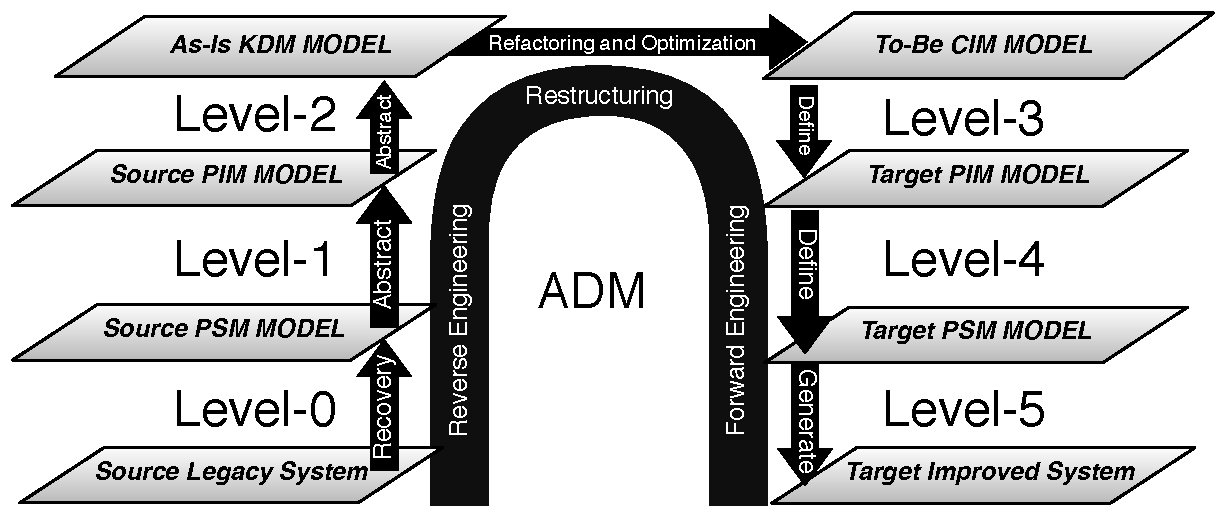
\includegraphics[width=11cm, height=3.8cm]{figure/processoDaFerramenta}
\caption{KDM-RE Process}
\label{fig:process}
\end{figure} 

After creating the PSM the next level (\textbf{Level-2}) consists in transforming the PSM to a Platform-Indented Model (PIM) which is based on the KDM. 
Therefore, in this level the KDM-RE performs a set of model-to-model transformation to get an instance of the KDM which represents the systems ``AS-IS''. 
These transformations are performed by ATL (ATL Transformation Language)\footnote{https://www.eclipse.org/atl/} along with MoDisco\footnote{http://www.eclipse.org/MoDisco/}.
Similarly, the KDM-RE also provides a popup menu named ``Discovery KDM Model'' which by clicking on it the engineer gets a instance of the KDM based on the earlier PSM.
In Figure~\ref{fig:discovery_kdm_model} depicts how to get the instance of the KDM.

\begin{figure}
\centering
\begin{minipage}{.5\textwidth}
  \centering
  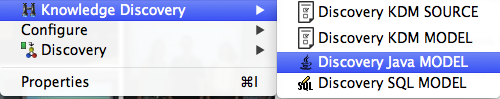
\includegraphics[width=6cm]{figure/discovery_java_model}
  \caption{Discovery Java Model}
  \label{fig:discovery_java_model}
\end{minipage}%
\begin{minipage}{.5\textwidth}
  \centering
  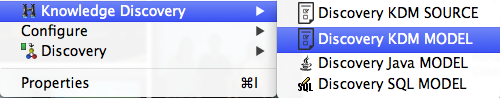
\includegraphics[width=6cm]{figure/discovery_kdm_model}
  \caption{Discovery KDM Model}
  \label{fig:discovery_kdm_model}
\end{minipage}
\end{figure}

In Figure~\ref{fig:interface} we depicted the main window of our \textit{plug-in}. 
For explanation purpose, we have identified main regions, i.e., \textcircled{a}, \textcircled{b}, \textcircled{c} and \textcircled{d}.

\begin{figure}[!ht]
\centering
  % Requires \usepackage{graphicx}
  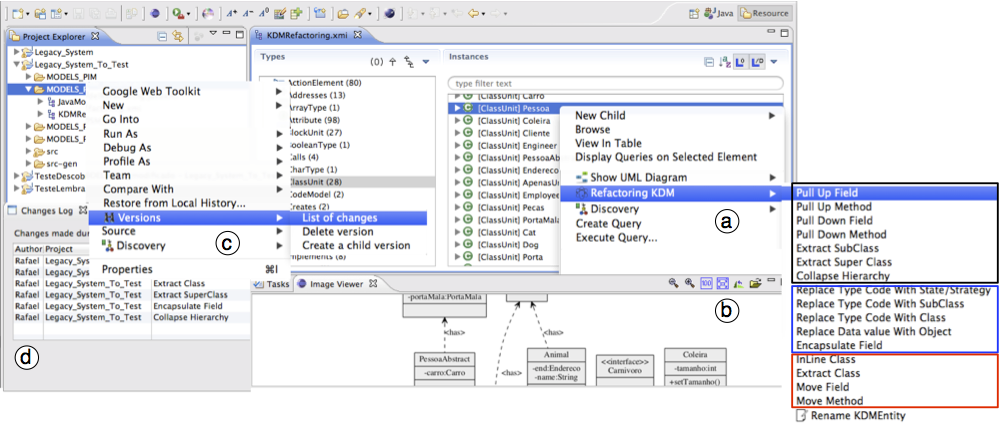
\includegraphics[width=15cm, height=6.8cm]{figure/ScreenShot_tool}
\caption{KDM-RE's Interface}
\label{fig:interface}
\end{figure}

After getting the KDM, the engineer can realize the refactorings.
In order to assist this activity, KDM-RE provides a popup menu which depicts all refactorings that can be carried out.
In the region \textcircled{a} (see Figure~\ref{fig:interface}) it is possible to select all 16 refactorings that have been implemented in KDM-RE. 
For illustration purposes only we drew rectangles to separate the refactorings into three groups. 
The black rectangle represents refactorings that deal with generalization, the blue rectangle stand for refactorings to organize data and the red one symbolize refactoring to assist the moving features between objects.

The region \textcircled{b} (see Figure~\ref{fig:interface}) shows a class diagram. This diagram is generated as the engineer performs the refactorings in KDM model, i.e., changes are reproduced on the fly in a class diagram.
We claim that this is important once the class diagram provides an abstract view of the system, hence, the engineer can visually check the system's changes after applying a set of refactorings. 
In addition, usually the source code is the only available artifact of the legacy software. 
Therefore, creating a class diagram makes, both the legacy software and the generated software to have a new type of artifact (i.e., UML class models), improving their documentation.

KDM-RE also supplies a multiple versions of a system at level models (KDM) which allows the engineer to work interactively on multiple models and to explore alternate refactoring path. As can see in the region \textcircled{c} (see Figure~\ref{fig:interface}), the engineer must select a KDM file, then he must right-click on the mouse to appear a popup menu named ``Versions''. By releasing the mouse on this menu, three options will show: (\textit{i}) List of changes, (\textit{ii}) Delete version and (\textit{iii}) Create a child version. The last option create a copy of the KDM file - then the engineer can explore another refactoring path. The second option delete a version and the first option shows all changes that have been realized in a current KDM file, all changes are depicted in an Eclipse View, as shown in region \textcircled{d}, as can be seen the changes.




